\documentclass[titlepage]{jarticle}
\usepackage[dvipdfmx]{graphicx}
\usepackage{listings}
\usepackage{here}
\usepackage{r04ec-exp}
%
\lstset{
  basicstyle={\ttfamily},
  identifierstyle={\small},
  commentstyle={\smallitshape},
  keywordstyle={\small\bfseries},
  ndkeywordstyle={\small},
  stringstyle={\small\ttfamily},
  frame={tb},
  breaklines=true,
  columns=[l]{fullflexible},
  numbers=left,
  xrightmargin=0zw,
  xleftmargin=3zw,
  numberstyle={\scriptsize},
  stepnumber=1,
  numbersep=1zw,
  lineskip=-0.5ex,
  language=c
}
\renewcommand{\lstlistingname}{ソースコード}
\makeatletter
\newcommand{\figcaption}[1]{\def\@captype{figure}\caption{#1}}
\newcommand{\tblcaption}[1]{\def\@captype{table}\caption{#1}}
\makeatother
%%% 表紙の記載事項設定
%
% 実験題目  ※レポートを書くときは,まず,タイトルを正しいものに変えましょう
%
\title{信号処理プログラミング}
% 学年・番号
\grade{4年37番}%
% 氏名
\author{本間 三暉}
% 班(後期は班に分かれて実験をする.そのときは,ここに班番号を記入する.)
\team{}
% 提出日
\date{2022年7月1日}
% 実験日
\expdate{2022年4月14日,4月21日,4月28日,5月19日}
% 共同実験者
% グループに分かれて実験をするテーマでは,グループメンバーの番号名前を書く.
\coauthor{%
}
%
%記載例:
%\coauthor{%
%  2番 & 新潟 花子\\
%  11番 & 三条 次郎}
%%
\begin{document}
\maketitle
\section{はじめに}
このレポートにおいて章,項,節番号は実験テキスト及び通常レポートと同期する形で作成する.なお,通常レポートと重複する部分は省略する.
\setcounter{section}{1}
\section{演習}
通常レポートで示した通りである.
また,通常レポートに示した定義ファイルにソースコード\ref{define}を追加した.
\begin{lstlisting}[caption=定義ファイル追加,label=define]
#define ROUND(x) ((x > 0) ? (x + 0.5) : (x - 0.5))
\end{lstlisting}
\subsection{次の指示に従いプログラムを作成し,出力を gnuplot で可視化して動作確認を行え}
\setcounter{subsubsection}{2}
\subsubsection{任意の弧度$r$に対して,矩形波の振幅値を求める関数squを作成せよ}
ソースコード\ref{squ}に関数squを示す.
\begin{lstlisting}[caption=double squ(double r),label=squ]
double squ(double r) {
  return ((saw(r) < 0) ? -1 : 1);
}
\end{lstlisting}
通常レポートで作成したsaw関数を流用し,saw(r)が正のときは1,そうでないときは$-1$を取るようにした.
原理的には数学関数のsin関数等を使用しても良いが,実行時間などの観点から,こっちの方が良いと判断した.

入力範囲を[$-2\pi:2\pi$]としたときの出力波形を図\ref{fig:squ}に示す.
\begin{figure}[H]
  \centering
  \includegraphics[width=7cm]{EPS/squ.eps}
  \caption{squの出力波形}
  \label{fig:squ}
\end{figure}

\subsubsection{任意の弧度rに対して,三角波の振幅値を求める関数triを作成せよ}
ソースコード\ref{tri}に示す.
\begin{lstlisting}[caption=double tri(double r),label=tri]
  double tri(double r) {
    int index = 1;
    double triangle, mod;

    mod = fmod(r, PI);
    if (r < 0) mod = mod + PI;
    triangle = mod * 2 / PI;

    if (triangle > 1) triangle = 2 - triangle;
    if (r < 0) {
      r *= (-1);
      index *= (-1);
    }

    while (1) {
      r -= PI;
      if (r < 0) break;
      index *= (-1);
    }
    triangle *= index;
    return triangle;
  }
\end{lstlisting}

入力範囲を[$-2\pi:2\pi$]としたときの出力波形を図\ref{fig:tri}に示す.
\begin{figure}[H]
  \centering
  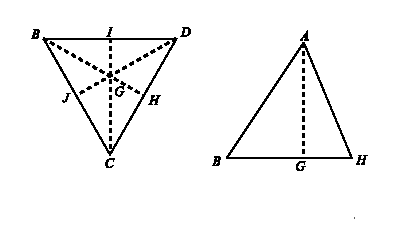
\includegraphics[width=7cm]{EPS/tri.eps}
  \caption{triの出力波形}
  \label{fig:tri}
\end{figure}

\subsection{次の指示に従いプログラムを作成し,動作を確認せよ.}
\setcounter{subsubsection}{2}
\subsubsection{量子化誤差を評価するため,sin10af1.cに量子化における二乗平均平方根誤差を計算する機能を追加せよ.}
ソースコード\ref{esum_main}にmain部の変更点,ソースコード\ref{esum_err_sum}に追加したユーザ定義関数を示す.

\begin{lstlisting}[caption=esumに関係するmain部の変更点,label=esum_main]
for (t = 0; t <= T_END; t += DT, n++) {
  rad = t / (1000 / frq) * 2 * PI;
  vin = amp * sin(rad) + A_BIAS;

  vout = (vin < 0) ? 0 : ((vin > 255) ? 225 : vin);
  esum = err_sum(vin, vout, esum);
  printf("%4d, %4d\n", t, vout);
}
esum /= n;
esum = sqrt(esum);
printf("#E %g\n", esum);
\end{lstlisting}
\begin{lstlisting}[caption=double err\_sum(double{,}unsigned char{,}double),label=esum_err_sum]
double err_sum(double true_value, unsigned char quantization, double e_rms) {
  e_rms = (true_value - quantization) * (true_value - quantization);
  return e_rms;
}
\end{lstlisting}
ソースコード\ref{esum_err_sum}は量子化前の値true\_valueと量子化後の値quantizationの差を二乗したものを戻り値とする関数である.

\subsubsection{各時刻の振幅値の小数点以下第一位を四捨五入して量子化するプログラムsin10af2.cを作成し,量子化におけるRMS誤差の軽減効果を定量的に調べよ.}
sin10af2.cのsin10af1.cからの変更点をソースコード\ref{sin10af2}に示す.
\begin{lstlisting}[caption=sin10af2.c,label=sin10af2]
  for (t = 0; t <= T_END; t += DT, n++) {
    rad = t / (1000 / frq) * 2 * PI;
    vin = amp * sin(rad) + A_BIAS;
    vout = (vin < 0) ? 0 : ((vin > 255) ? 225 : ROUND(vin));
    esum = err_sum(vin, vout, esum);
    printf("%4d, %4d\n", t, vout);
  }
\end{lstlisting}
ソースコード\ref{sin10af2}はvinの値をvoutに代入するときに四捨五入をするようにしたものである.
sin10af1.cにソースコード\ref{esum_main}の変更を加えたファイルとsin10af2.cに振幅100,周波数3[Hz]の条件で時系列データのRMS誤差を比べると,図\ref{esum}のようになる.
\begin{table}[H]
  \caption{四捨五入によるRMS誤差の比較}
  \label{esum}
  \centering
  \begin{tabular}{c|cc}\hline
              & sin10af1    & sin100af2               \\\hline\hline
    $E_{RMS}$ & $0.0995037$ & $7.07016\times10^{-15}$ \\\hline
  \end{tabular}
\end{table}
これらの値を比較すると$10^{13}$倍の差があることがわかる.四捨五入をすることでRMS誤差が大幅に軽減されたことが確認できる.

\setcounter{subsubsection}{5}
\subsubsection{正弦波の振幅,周波数,位相,標本化間隔(ms単位の実数)をコマンドライン引数で指定したとき,サンプリング結果を出力するプログラムを作成せよ.}
位相の単位をms単位の実数としたときのソースコードをソースコード\ref{sinafpt}に示す.
なお,位相角の単位はSI単位系ではラジアン(rad)であるが,
今回は波形が正しいか確認しやすいため,単位はms単位の実数とする.
\begin{lstlisting}[caption=sinafpt.c,label=sinafpt]
  int main(int argc, char **argv) {
    int t, n = 0;
    double amp, frq, phf, rad, vin, esum = 0, dt;
    unsigned char vout;
  
    if (argc != 5) {
      fprintf(stderr, "Usage: %s amplitude frequency\n", argv[0]);
      return EXIT_FAILURE;
    }
  
    amp = atof(argv[1]);
    frq = atof(argv[2]);
    phf = atof(argv[3]);
    dt = atof(argv[4]);

    printf("#A %f\n", amp);
    printf("#F %f\n", frq);
    printf("#T %f\n", dt);
    printf("#B %d\n", A_BIAS);
    printf("#N %f\n", T_END / dt + 1);
  
    for (t = 0; t <= T_END; t += dt) {
      rad = (t + phf) / (1000 / frq) * 2 * PI;
      vin = amp * sin(rad) + A_BIAS;
      vout = (vin < 0) ? 0 : ((vin > 255) ? 225 : ROUND(vin));
      printf("%4d, %4d\n", t, vout);
    }
    return EXIT_SUCCESS;
  }
\end{lstlisting}
これを用いて,振幅100,周波数10[Hz],位相25[ms],標本化間隔3[ms]の正弦波を出力したものを図\ref{fig:sinafpt}に示す.
波形を見やすくするため,実際には1000[ms]まで測定したが,横軸は[0:600]の範囲で出力する.

入力した条件から,周波数10[Hz]のとき1周期は100[ms]となる.位相はこれの$\frac{1}{4}$倍の25[ms]なので,振幅100,周波数10[Hz],標本化間隔3[ms]の余弦波が出力されていればよいはずである.
図\ref{fig:sinafpt}を見ると,振幅100,周波数10[Hz],標本化間隔3[ms]の余弦波が出力されているため正しいことが確認できる.

\subsubsection{振幅,周波数,位相,標本化間隔(ms単位の実数)をコマンドライン引数で指定したとき,のこぎり波,矩形波,三角波を出力するプログラムを作成せよ.}
プログラムsin10af2の主要部ソースコード\ref{sin10af2}をソースコード\ref{sawaft},\ref{squaft},\ref{triaft}に書き換えることで,それぞれのこぎり波,矩形波,三角波を出力するプログラムを示す.
\begin{lstlisting}[caption=sawaft.c,label=sawaft]
  dt = atof(argv[3]);
  printf("#N %f\n", T_END / dt + 1);

  for (t = 0; t <= T_END; t += dt) {
    rad = t / (1000 / frq) * 2 * PI;
    vin = amp * saw(rad) + A_BIAS;
    vout = (vin < 0) ? 0 : ((vin > 255) ? 225 : ROUND(vin));
    printf("%4f, %4d\n", t, vout);
  }
\end{lstlisting}
\begin{lstlisting}[caption=squaft.c,label=squaft]
  dt = atof(argv[3]);
  printf("#N %f\n", T_END / dt + 1);

  for (t = 0; t <= T_END; t += dt) {
    rad = t / (1000 / frq) * 2 * PI;
    vin = amp * squ(rad) + A_BIAS;
    vout = (vin < 0) ? 0 : ((vin > 255) ? 225 : ROUND(vin));
    printf("%4f, %4d\n", t, vout);
  }
\end{lstlisting}
\begin{lstlisting}[caption=triaft.c,label=triaft]
  dt = atof(argv[3]);
  printf("#N %f\n", T_END / dt + 1);

  for (t = 0; t <= T_END; t += dt) {
    rad = t / (1000 / frq) * 2 * PI;
    vin = amp * tri(rad) + A_BIAS;
    vout = (vin < 0) ? 0 : ((vin > 255) ? 225 : ROUND(vin));
    printf("%4f, %4d\n", t, vout);
  }
\end{lstlisting}
これらのソースコードに振幅100,周波数3[Hz],標本化間隔3[ms]の条件で出力した波形を図\ref{fig:sawaft},\ref{fig:squaft},\ref{fig:triaft}に示す.

\begin{figure}[H]
  \begin{minipage}{0.495\hsize}
    \centering
    \includegraphics[width=7cm]{EPS/sinafpt.eps}
    \caption{sinafpt.cで出力した正弦波}
    \label{fig:sinafpt}
  \end{minipage}
  \begin{minipage}{0.495\hsize}
    \centering
    \includegraphics[width=7cm]{EPS/sawaft.eps}
    \caption{sawaft.cで出力したのこぎり波}
    \label{fig:sawaft}
  \end{minipage}
  \begin{minipage}{0.495\hsize}
    \centering
    \includegraphics[width=7cm]{EPS/squaft.eps}
    \caption{squaft.cで出力した矩形波}
    \label{fig:squaft}
  \end{minipage}
  \begin{minipage}{0.495\hsize}
    \centering
    \includegraphics[width=7cm]{EPS/triaft.eps}
    \caption{triaft.cで出力した三角波}
    \label{fig:triaft}
  \end{minipage}
\end{figure}
グラフの範囲は[0:999]である.
これらの波形を見る限り出力されていることが確認できる.
\subsection{次のプログラムを作成して動作を確認せよ.出力の形式はプログラム例3を参考にして,加工後の振幅値を一列加えることにしておくと良い.}
\setcounter{subsubsection}{2}
\subsubsection{5点単純移動平均プログラムを作成せよ}
5点単純移動平均プログラムのオンライン型をソースコード\ref{5point:1}に,オフライン型をソースコード\ref{5point:2}に示す.
\begin{lstlisting}[caption=mvave5-1.c,label=5point:1]
  #define MOVING_AVERAGE 5
  int main(int argc, char **argv) {
    int tm, ain, aout, nmax, n = 0;
    double err_5add = 0.0, now;
    char buf[BUFSIZE];
    int err_before[MOVING_AVERAGE];
    FILE *fp;
  
    if (argc != 2) {
      fprintf(stderr, "Usage: %s infile max_noise\n", argv[0]);
      return EXIT_FAILURE;
    }
    if ((fp = fopen(argv[1], "r")) == NULL) {
      fprintf(stderr, "File: %s cannot open\n", argv[1]);
      return EXIT_FAILURE;
    }
    while (fgets(buf, sizeof(buf), fp) != NULL) {
      if (buf[0] == '#') {              
        printf("%s", buf);
        continue;
      }
      tm = atoi(strtok(buf, ","));
      ain = atoi(strtok(NULL, "\r\n\0"));
      for (int count = MOVING_AVERAGE - 1; count > 0; count--) {
        err_before[count] = err_before[count - 1];

      }
      err_before[0] = ain / MOVING_AVERAGE;
      err_5add += err_before[0];
      if (n < MOVING_AVERAGE - 1) {
        n++;
        continue;
      }
      aout = (err_5add < 0) ? 0 : (err_5add > 255) ? 225 : ROUND(err_5add);
  
  #if defined TEST
      printf("%4d, %4d, %4d\n", tm, ain, aout);
  #else
      printf("%4d,%4d\n", tm, aout);
  #endif
      err_5add -= err_before[MOVING_AVERAGE - 1];
    }
    fclose(fp);
    return EXIT_SUCCESS;
  }
\end{lstlisting}
\begin{lstlisting}[caption=mvave5-2.c,label=5point:2]
  #define MOVING_AVERAGE 5
  int main(int argc, char **argv) {
    int n, i;
    int tm[DATANUM], amp[DATANUM], aout[DATANUM] = {0}, editing[DATANUM - 1];
    int nmax;
    double err, err_5add = 0;
    char buf[BUFSIZE];
    FILE *fp;
  
    if (argc != 2) {
      fprintf(stderr, "Usage: %s infile max_noise\n", argv[0]);
      return EXIT_FAILURE;
    }
    if ((fp = fopen(argv[1], "r")) == NULL) {
      fprintf(stderr, "File: %s cannot open\n", argv[1]);
      return EXIT_FAILURE;
    }
    for (n = 0; n < DATANUM;) {
      if (fgets(buf, sizeof(buf), fp) == NULL) break;
      if (buf[0] == '#') {
        printf("%s", buf);
        continue;
      }
      tm[n] = atoi(strtok(buf, ","));
      amp[n] = atoi(strtok(NULL, "\r\n\0")) / MOVING_AVERAGE;
      n++;
    }
    fclose(fp);
    for (n = 0; n < MOVING_AVERAGE - 1; n++) {
      err_5add += amp[n];
    }
    for (n = MOVING_AVERAGE / 2-1; n <= DATANUM - 1; n++) {
      err_5add += amp[n + MOVING_AVERAGE / 2];
      aout[n] = (err_5add < 0) ? 0 : (err_5add > 255) ? 225 : ROUND(err_5add);
      err_5add -= amp[n - MOVING_AVERAGE / 2];
    }
    for (n = MOVING_AVERAGE / 2-1; n <= DATANUM - (MOVING_AVERAGE / 2); n++) {
  #if defined TEST
      printf("%4d, %4d, %4d\n", tm[n], amp[n] * MOVING_AVERAGE, aout[n]);
  #else
      printf("%4d,%4d\n", tm[n], aout[n]);
  #endif
    }
    return EXIT_SUCCESS;
  }
\end{lstlisting}
予めデータを4つの合計を求めておき,新しいデータを読み込むたびにそれに加算し平均を求める.
その後加算した中で最も古いデータを引くことで一度のループに対して,一回の加算,一回の除算,一回の減算で計算を行うことができる.
これらに,振幅100,周波数3[Hz]の正弦波に最大値を10に設定した白色雑音を加えた波形と,それに5点移動平均処理を施した波形を比較する.
オンライン型によって処理したものを図\ref{fig:5point:1}に,オフライン型によって処理したものを図\ref{fig:5point:2}に示す.
\begin{figure}[H]
  \begin{minipage}{0.495\hsize}
    \centering
    \includegraphics[width=7cm]{EPS/mvave5-1.eps}
    \caption{オンライン型で処理した振幅100,周波数3[Hz],最大白色雑音10の正弦波}
    \label{fig:5point:1}
  \end{minipage}
  \begin{minipage}{0.495\hsize}
    \centering
    \includegraphics[width=7cm]{EPS/mvave5-2.eps}
    \caption{オフライン型で処理した振幅100,周波数3[Hz],最大白色雑音10の正弦波}
    \label{fig:5point:2}
  \end{minipage}
\end{figure}
これを見ると,オンライン型はオフライン型に比べ値を出力するのに遅れが生じていることがわかる.また,最大振幅が小さくなっているように感じる.
これを確かめるため,振幅100,周波数3[Hz]の正弦波に最大値を10に設定した白色雑音を加えた波形を3点移動平均と5点移動平均で処理したものを比較する.
それを図\ref{周央サンゴ}に示す.なお,オンライン型とオフライン型には出力時間のズレ以外の違いがないので,両方ともオフライン型の場合のみを比較する.
\begin{figure}[H]
  \centering
  \includegraphics[width=7cm]{EPS/3-5.eps}
  \caption{3点移動平均及び5点移動平均の比較}
  \label{周央サンゴ}
\end{figure}
図\ref{周央サンゴ}を見ると波形の振幅値が大きくなるにつれ,3点移動平均は5点移動平均に比べ振幅値は小さくなっている事がわかる.
この事実は,3点移動平均と5点移動平均のどちらが優れているかを判断するときの一つの指標になると考えられる.

\subsection{次の指示に従い,式変形及びプログラム作成と動作確認を行え.}

\setcounter{subsubsection}{2}
\subsubsection{雑音が重畳されたCSVファイルを引数として与えたときに,SNR[dB]を求めるプログラムを作成せよ.}\label{snr1}
SNR[dB]を求めるプログラムの主要部をソースコード\ref{snr1.c}に示す.
\begin{lstlisting}[caption=snr1.cの主要部,label=snr1.c]
  while (fgets(buf, sizeof(buf), fp) != NULL) {
    if (buf[0] == '#') {
      printf("%s", buf);
      continue;
    }
    tm[n] = atoi(strtok(buf, ","));
    amp[n] = atoi(strtok(NULL, ","));
    aerr[n] = atoi(strtok(NULL, "\r\n\0"));
    add_s += (amp[n] - A_BIAS) * (amp[n] - A_BIAS);
    add_n += (aerr[n] - amp[n]) * (aerr[n] - amp[n]);
    n++;
  }
  snr_db = 10 * log10(add_s / add_n);
\end{lstlisting}
振幅100,周波数3[Hz],白色雑音の最大値を10とした正弦波を基本波形として,その波形から振幅,周波数,白色雑音の最大値の値の内それぞれ一つだけ変えた波形を作成する.
それぞれの値を振幅140,周波数5[Hz],白色雑音の最大値15としたとき4つのデータを比較したものを表\ref{tab:snr1}に示す.

%ここに表
\begin{table}[H]
  \caption{白色雑音を加えた波形のS/N比}
  \label{tab:snr1}
  \centering
  \begin{tabular}{l|cccc}\hline
          & 基本波形  & 振幅140   & 周波数5{[}Hz{]} & 白色雑音の最大値15 \\\hline\hline
    S/N比 & 22.929221 & 26.120139 & 23.190504       & 19.768701
  \end{tabular}
\end{table}

毎回シード値がランダムな疑似乱数を使用しているため.多少の誤差は発生してしまうため許容しなくてはならない.
しかし,表\ref{tab:snr1}を見ると,白色雑音の最大値を変えた場合のS/N比の変化量が比較的大きい.そのため主にS/N比は白色雑音の最大値によって変化量が変化すると考えられる.

\subsubsection{3点移動平均や5点移動平均を行った後のCSVファイルを引数として与えたときに,SNR[dB]を求めるプログラムを作成せよ.}\label{snr2}
もとの波形を出力したCSVファイルと,3点移動平均,及び5点移動平均を行った後のファイルをコマンドライン引数によって与えることとする.
SNR[dB]を求めるプログラムをソースコード\ref{snr2.c}に示す.
このソースコードをオフライン型にした理由として,移動平均プログラムを行うことでデータ数が減ってしまうため,一つのループで完結させるのが難しい点が挙げられる.

ここで注意しなければならないのが,もとの波形に比べ,3点移動平均や5点移動平均処理を行った後ではデータ数が少なくなっている点である.
今回は2つのファイルからそれぞれ雑音を加える前の波形データと,移動平均によって雑音を抑える処理をした波形データを読み取ったが,
コメント行に波形の情報があり生成する波のおおよその形がわかっていれば,ソースコード\ref{snr_hoge}のようにして波形を生成することもできる.
\begin{lstlisting}[caption=snr2.cの主要部,label=snr2.c]
  adjustment = atoi(argv[3]);
  while (fgets(buf2, sizeof(buf2), fp2) != NULL) {
    if (buf2[0] == '#') {
      printf("%s", buf2);
      continue;
    }
    tm[sn] = atoi(strtok(buf2, ","));

    aerr[sn] = atoi(strtok(NULL, ","));
    amp[sn] = atoi(strtok(NULL, "\r\n\0"));
    add_s += (amp[sn] - A_BIAS) * (amp[sn] - A_BIAS);
    sn++;
  }
  nn = adjustment / 2;
  while (fgets(buf1, sizeof(buf1), fp1) != NULL) {
    if (buf1[0] == '#') {
      printf("%s", buf1);
      continue;
    }
    tm[nn] = atoi(strtok(buf1, ","));

    aerr[nn] = atoi(strtok(NULL, ","));
    edit[nn] = atoi(strtok(NULL, "\r\n\0"));
    add_n += (edit[nn] - amp[nn]) * (edit[nn] - amp[nn]);
    nn++;
  }
  snr_db = 10 * log10((add_s / sn) / (add_n / (nn - adjustment / 2)));
  printf("%f", snr_db);
\end{lstlisting}
\begin{lstlisting}[caption=波形情報が既知の場合のsnr2.cの主要部,label=snr_hoge]
  while (fgets(buf, sizeof(buf), fp) != NULL) {
  if (buf[0] == '#') {
    printf("%s", buf);
    if (buf[1] == 'A') {
      ampli = atoi(strtok((buf + 3), "\r\n\0"));
    } else if (buf[1] == 'F') {
      frq = atoi(strtok((buf + 3), "\r\n\0"));
    }
    continue;
  }
  tm[n] = atoi(strtok(buf, ","));

  rad = tm[n] / (1000 / (double)frq) * 2 * PI;

  amp[n] = (double)ampli * sin(rad) + A_BIAS;

  aerr[n] = atoi(strtok(NULL, ","));
  edit[n] = atoi(strtok(NULL, "\r\n\0"));

  add_s += (amp[n] - A_BIAS) * (amp[n] - A_BIAS);
  add_n += (edit[n] - amp[n]) * (edit[n] - amp[n]);
  n++;
}
\end{lstlisting}
\ref{snr1}で作成した雑音が重畳されたCSVファイルを3点移動平均,及び5点移動平均を取り,それぞれのS/N比を求める.求めたS/N比をまとめたものを表\ref{tab:snr2}に示す.
\begin{table}[H]
  \caption{3点移動平均及び5点移動平均を取った値のS/N比とその変化量}
  \label{tab:snr2}
  \centering
  \begin{tabular}{l|cccc}\hline
                            & 基本波形  & 振幅140   & 周波数5{[}Hz{]} & 白色雑音の最大値15 \\\hline\hline
    3点移動平均             & 36.767451 & 35.558365 & 29.260603       & 36.767451          \\
    5点移動平均             & 27.264763 & 27.111184 & 19.574977       & 27.264763          \\
    3点移動平均による変化量 & 13.83823  & 9.438226  & 6.070099        & 16.99875           \\
    5点移動平均による変化量 & 4.335542  & 0.991045  & -3.615527       & 7.496062           \\\hline
  \end{tabular}
\end{table}
これを見ると,おおよそ5点移動平均より3点移動平均のほうがS/N比が大きくなることがわかる.つまり,3点移動平均の方がより雑音を取り除けていると考えられる.
移動平均処理を行うと,もとの波形と比べ振幅値が小さくなる.これはもとの波形の振幅が大きくなるほど影響を受けやすい.
周波数5[Hz]のときのS/N比が小さいが,これは振幅値が最も大きくなる地点のサンプルをより多く採取してしまっているからではないかと考えられる.
このデータを見ると,3点移動平均の方が5点移動平均よりS/N比が大きくなっているため3点移動平均のほうが優れていると考えることができる.
\subsection{以下の指示に従って,プログラミングと動作確認を行え.}
\setcounter{subsubsection}{2}
\subsubsection{ステレオ音声・量子化ビット数16のWAVEファイルの波形データをCSVファイルに出力するダンププログラムを作成せよ.}
ステレオ音声・量子化ビット数16のWAVEファイルの波形データをCSVファイルに出力するダンププログラムをソースコード\ref{wav2txt-s16.c}に示す.
\begin{lstlisting}[caption=wav2txt-s16.c,label=wav2txt-s16.c]
  uLong read_head(FILE *fp, uShort *ch, uShort *qbit) {
    char str[H_LEN];
    uLong riffsize, fmtsize, smprate, datasize, bytepersec;
    uShort fid, blksize;
  
    fread(str, sizeof(char), H_LEN, fp);
    if (memcmp("RIFF", str, H_LEN) != 0) return 0;
    fread(&riffsize, sizeof(uLong), 1, fp);
    printf("# RIFF size: %ld\n", riffsize);
    fread(str, sizeof(char), H_LEN, fp);
    if (memcmp("WAVE", str, H_LEN) != 0) return 0;
    fread(str, sizeof(char), H_LEN, fp);
    if (memcmp("fmt ", str, H_LEN) != 0) return 0;
    fread(&fmtsize, sizeof(uLong), 1, fp);
    printf("# fmt size: %ld\n", fmtsize);
    fread(&fid, sizeof(uShort), 1, fp);
    printf("# fmt ID: %d\n", fid);
    if (fid != ID_LPCM) return 0;
    fread(ch, sizeof(uShort), 1, fp);
    printf("# CH: %d\n", *ch);
    fread(&smprate, sizeof(uLong), 1, fp);
    printf("# Sampling rate: %ld\n", smprate);
    fread(&bytepersec, sizeof(uLong), 1, fp);
    printf("# Bytes per sec: %ld\n", bytepersec);
    fread(&blksize, sizeof(uShort), 1, fp);
    printf("# Block size: %d\n", blksize);
    fread(qbit, sizeof(uShort), 1, fp);
    printf("# Q bit: %d\n", *qbit);
    fread(str, sizeof(char), H_LEN, fp);
    if (memcmp("data", str, H_LEN) != 0) return 0;
    fread(&datasize, sizeof(uLong), 1, fp);
    printf("# datasize: %ld\n", datasize);
    return smprate;
  }
  
  int main(int argc, char **argv) {
    double count;
    double tm = 0;
    short datR, datL;
    long start_num = 0L, end_num;
    FILE *fp;
    uLong dsize, sampling_rate;
    uShort ch, qbit;
  
    if (argc < 2) {
      fprintf(stderr, "Usage: %s file page\n", argv[0]);
      return EXIT_FAILURE;
    }
    if ((fp = fopen(argv[1], "rb")) == NULL) {
      fprintf(stderr, "File (%s) cannot open\n", argv[1]);
      return EXIT_FAILURE;
    }
  
    sampling_rate = read_head(fp, &ch, &qbit);
    if (argc > 3) {
      start_num = atol(argv[2]) * (qbit / 8) * ch;
      fseek(fp, start_num, SEEK_CUR);
    }
    if (argc == 4) {
      end_num = atoi(argv[3]);
    } else {
      end_num = sampling_rate;
    }
    tm = (double)start_num / sampling_rate * 1000.0;
    count = 1000.0 / sampling_rate;

    while (fread(&datL, sizeof(short), 1, fp)) {
      if (!(fread(&datR, sizeof(short), 1, fp))) break;

      tm += count;
      printf("%0.3f,%4d,%4d\n", tm, datL, datR);
      if (tm > end_num) break;
    }
    fclose(fp);
    return EXIT_SUCCESS;
  }
\end{lstlisting}
ここで注意しなければならないのが,今回量子化ビット数が16なので,取り出した波形はshort型に格納しなければいけない.

仮にunsigned char型で取り出すと図\ref{chimes_char},int型に格納すると図\ref{chimes_int},unsigned short型に格納すると図\ref{chimes_uShort}のようになる.
基本的にLの値もRの値も2バイトでないと表せない値が入っているためデータ数が1バイトしかないchar型に合わせ1バイトずつ値を取得すると元の値が負の値を取る場合や255以下の値を持つときに0や255などの振り切れた値を出力してしまう.

2バイトで取り出した値を4バイトで表されるint型に格納する際,最下位ビットから数えて必要な分しか書き換えないため,今回だと最上位ビットから数えて8ビット分の値がわからずN/Aとなる.

また,unsigned short型の変数に値を格納する場合,本来負の値を取るはずのデータが別の正の値を取ってしまうため負の値の部分が上にスライドしたような形になっている.

ソースコード\ref{wav2txt-s16.c}のダンププログラムを使用して,出力したchimes.wavの波形を図\ref{chimes.wav}に示す.
\begin{figure}[H]
  \begin{minipage}{0.495\hsize}
    \centering
    \includegraphics[width=7cm]{EPS/chimes_char.eps}
    \caption{unsigned char型に収まるように波形データを取り出したchimes.wavの波形}
    \label{chimes_char}
  \end{minipage}
  \begin{minipage}{0.495\hsize}
    \centering
    \includegraphics[width=7cm]{EPS/chimes_int.eps}
    \caption{取り出した波形データをint型の変数に格納したchimes.wavの波形}
    \label{chimes_int}
  \end{minipage}
  \begin{minipage}{0.495\hsize}
    \centering
    \includegraphics[width=7cm]{EPS/chimes_uShort.eps}
    \caption{取り出した波形データをunsigned short型の変数に格納chimes.wavの波形}
    \label{chimes_uShort}
  \end{minipage}
  \begin{minipage}{0.495\hsize}
    \centering
    \includegraphics[width=7cm]{EPS/chimes.eps}
    \caption{chimes.wavの出力波形}
    \label{chimes.wav}
  \end{minipage}
\end{figure}
細かく振動することで波による上下差をなくし,比較的音のゆらぎの少ないファイルを作っているのだと思われる.
また,図\ref{chimes.wav}を見ると,振幅の大きさがLとRでほんの少し違うことがわかる.
これはLとRで少し違う大きさの音を出し,音に立体感を出しているのだと思われる.

\section{課題}
ここではソースコード\ref{task_header}に示すようなヘッダファイルが読み込まれているものとする.
\begin{lstlisting}[caption=課題のヘッダファイル,label=task_header]
  #define T_END 1000
  #define DT 1
  #define A_BIAS 0x80
  #define FRQ 3
\end{lstlisting}
周期関数$f_{1}$,$f_{2}$,$f_{3}$を実装したプログラムをそれぞれソースコード\ref{f_1},\ref{f_2},\ref{f_3}に示す.
\begin{lstlisting}[caption=周期関数$f_{1}(t)$の主要部,label=f_1]
  amp = atoi(argv[1]);

  m = atoi(argv[2]);
  for (int t = 0; t <= T_END; t += DT) {
    rad = t * FRQ * 2 * PI / 1000;
    f_1 = 0;
    for (count = 1; count <= m; count++) {
      f_1 += sin(count * rad) / count;
    }
    f_1 = 2 / PI * amp * f_1 + A_BIAS;
    printf("%4d,%4d\n", t, (int)f_1);
  }
\end{lstlisting}
\begin{lstlisting}[caption=周期関数$f_{2}(t)$の主要部,label=f_2]
  amp = atoi(argv[1]);

  m = atoi(argv[2]);
  for (int t = 0; t <= T_END; t += DT) {
    rad = t * FRQ * 2 * PI / 1000;
    f_2 = 0;
    for (count = 1; count < m; count++) {
      f_2 += sin((2 * count - 1) * rad) / (2 * count - 1);
    }
    f_2 = 4 / PI * amp * f_2 + A_BIAS;
    printf("%f,%f\n", rad, f_2);
  }
\end{lstlisting}
\begin{lstlisting}[caption=周期関数$f_{3}(t)$の主要部,label=f_3]
  amp = atoi(argv[1]);

  m = atoi(argv[2]);
  for (int t = 0; t <= T_END; t += DT) {
    rad = t * FRQ * 2 * PI / 1000;
    f_3 = 0;
    for (count = 1; count < m; count++) {
      f_3 += sin(count * PI / 2) * sin(count * rad) / (count * count);
    }
    f_3 = 2 / (PI * PI) * amp * f_3 + A_BIAS;
    printf("%f,%f\n", rad, f_3);
  }
\end{lstlisting}
これらのソースコードに振幅100として,試行回数 m が1,10,100,10000の場合について波形を出力する.
周期関数$f_{1}(t)$,$f_{2}(t)$,$f_{3}(t)$の波形をそれぞれ\ref{f_1:fig},\ref{f_2:fig},\ref{f_3:fig}に示す.
\begin{figure}[H]
  \begin{minipage}{0.495\hsize}
    \centering
    \includegraphics[width=7cm]{EPS/task_1.eps}
    \caption{振幅100,周波数3[Hz]の周期関数$f_{1}(t)$}
    \label{f_1:fig}
  \end{minipage}
  \begin{minipage}{0.495\hsize}
    \centering
    \includegraphics[width=7cm]{EPS/task_2.eps}
    \caption{振幅100,周波数3[Hz]の周期関数$f_{2}(t)$}
    \label{f_2:fig}
  \end{minipage}
  \begin{minipage}{0.495\hsize}
    \centering
    \includegraphics[width=7cm]{EPS/task_3.eps}
    \caption{振幅100,周波数3[Hz]の周期関数$f_{3}(t)$}
    \label{f_3:fig}
  \end{minipage}
\end{figure}
これらを見ると,$m=10$のときは振動している様子がよく分かる.また,$m=100$のときは殆どの場所で値が収束していて,極値付近のみ振動している様子が確認できる.
極値の波形を観察するため,$[0:10]$の範囲を切り出した波形をそれぞれ図\ref{f_1_10:fig},\ref{f_2_10:fig},\ref{f_3_10:fig}に示す.
\begin{figure}[H]
  \begin{minipage}{0.495\hsize}
    \centering
    \includegraphics[width=7cm]{EPS/task_1_10.eps}
    \caption{$[0:10]$の振幅100,周波数3[Hz]の周期関数$f_{1}(t)$}
    \label{f_1_10:fig}
  \end{minipage}
  \begin{minipage}{0.495\hsize}
    \centering
    \includegraphics[width=7cm]{EPS/task_2_10.eps}
    \caption{$[0:10]$の振幅100,周波数3[Hz]の周期関数$f_{2}(t)$}
    \label{f_2_10:fig}
  \end{minipage}
  \begin{minipage}{0.495\hsize}
    \centering
    \includegraphics[width=7cm]{EPS/task_3_10.eps}
    \caption{$[0:10]$の振幅100,周波数3[Hz]の周期関数$f_{3}(t)$}
    \label{f_3_10:fig}
  \end{minipage}
\end{figure}
これらを見ると$m=100$のとき,極値付近で減衰振動を行っていることがよくわかる.
mの値が増えるほど,理想的な波形に近づいていることがわかる.
$m=10000$の時のそれぞれの波形に最大値を10に設定した白色雑音を加えS/N比を求める.
また,雑音を加えた波形を3点移動平均と5点移動平均プログラムを用いて雑音を除去し,これらと元の波形のS/N比を求める.
求めたS/N比を表\ref{tab:task}にまとめる.
\begin{table}[H]
  \caption{周期関数$f_{i}(t)$のS/N比}
  \label{tab:task}
  \centering
  \begin{tabular}{l|cccc}\hline
                            & $f_{1}$   & $f_{2}$   & $f_{3}$   \\\hline\hline
    S/N比                   & 20.835381 & 25.806504 & 21.125344 \\
    3点移動平均             & 24.380427 & 29.52961  & 41.946036 \\
    5点移動平均             & 25.66529  & 30.426056 & 28.962362 \\
    3点移動平均による変化量 & 3.545046  & 3.723106  & 20.820692 \\
    5点移動平均による変化量 & 4.829909  & 4.619552  & 7.837018  \\\hline
  \end{tabular}
\end{table}
これを見ると,$f_{1}$,$f_{2}$は3点移動平均と5点移動平均の除去性能に大きな差は見られないが,$f_{3}$では圧倒的に3点移動平均の値が大きくなっている.
そのため,\ref{snr2}の結果もと合わせて考えると,3点移動平均のほうが優れていると考えることができる.
\section{発展課題}
モノラル音声のWAVEファイルをステレオ音声のWAVEファイルに変換するプログラムを作成した.
このプログラムをソースコード\ref{final_task.c}に示す.

なお,入力として量子化ビット数8のモノラル音声のWAVEファイルとそれをステレオ音声に変換して出力するためのWAVEファイルを与え,LからRに対して遅らせる位相の大きさはマクロ定義によって与えるものとする.
また,変換後の量子化ビット数は8とし,ずらした後の空いてしまったRの値は0とする.
\begin{lstlisting}[caption=発展課題,label=final_task.c]
  #include <ctype.h>
  #include <math.h>
  #include <stdio.h>
  #include <stdlib.h>
  #include <string.h>
  
  #define H_LEN 4 
  #define ID_LPCM 1 
  #define CH 2 
  #define DT 4 
  typedef unsigned short uShort;
  typedef unsigned long uLong;

  uLong header_data(FILE *fp, FILE *fp_write, short *q_bit, int *data_size) {
    char str[H_LEN];
    unsigned int h_len = H_LEN;
    uLong riff_size, fmt_size, sampling_rate, data_speed;
    uShort fid, block_size, ch;
  
    fread(str, sizeof(char), h_len, fp);
    if (memcmp("RIFF", str, h_len) != 0) return 0;
    fread(&riff_size, sizeof(uLong), 1, fp);
    printf("# RIFF size: %ld\n", riff_size);
    fread(str, sizeof(char), h_len, fp);
    if (memcmp("WAVE", str, h_len) != 0) return 0;
    fread(str, sizeof(char), h_len, fp);
    if (memcmp("fmt ", str, h_len) != 0) return 0;
    fread(&fmt_size, sizeof(uLong), 1, fp);
    printf("# fmt size: %ld\n", fmt_size);
    fread(&fid, sizeof(uShort), 1, fp);
    printf("# fmt ID: %d\n", fid);
    if (fid != ID_LPCM) return 0;
    fread(&ch, sizeof(uShort), 1, fp);
    printf("# CH: %d\n", ch);
    fread(&sampling_rate, sizeof(uLong), 1, fp);
    printf("# Sampling rate: %ld\n", sampling_rate);
    fread(&data_speed, sizeof(uLong), 1, fp);
    printf("# Bytes per sec: %ld\n", data_speed);
    fread(&block_size, sizeof(uShort), 1, fp);
    printf("# Block size: %d\n", block_size);
    fread(q_bit, sizeof(uShort), 1, fp);
    printf("# Q bit: %d\n", *q_bit);
    fread(str, sizeof(char), h_len, fp);
    if (memcmp("data", str, h_len) != 0) return 0;
    fread(data_size, sizeof(uLong), 1, fp);
    printf("# datasize: %ld\n", *data_size);
    *data_size *= 2;
    ch = CH;
    fwrite("RIFF", sizeof(char), 4, fp_write);
    fwrite(&riff_size, sizeof(int), 1, fp_write);
    fwrite("WAVE", sizeof(char), 4, fp_write);
    fwrite("fmt ", sizeof(char), 4, fp_write);
    fwrite(&fmt_size, sizeof(int), 1, fp_write);
    fwrite(&fid, sizeof(short), 1, fp_write);
    fwrite(&ch, sizeof(short), 1, fp_write);
    fwrite(&sampling_rate, sizeof(int), 1, fp_write);
    fwrite(&data_speed, sizeof(int), 1, fp_write);
    fwrite(&block_size, sizeof(short), 1, fp_write);
    fwrite(q_bit, sizeof(short), 1, fp_write);
    fwrite("data", sizeof(char), 4, fp_write);
    fwrite(data_size, sizeof(int), 1, fp_write);
    return sampling_rate;
  }
  
  int main(int argc, char **argv) {
    int sampling_rate, count = 0, data_size;
    unsigned short data_dt[DT] = {0};
    unsigned short datL, datR;
    uShort q_bit;
    FILE *fp;
    FILE *fp_write;
    if (argc < 2) {
      fprintf(stderr, "Usage: %s file page\n", argv[0]);
      return EXIT_FAILURE;
    }
    if ((fp = fopen(argv[1], "rb")) == NULL) {
      fprintf(stderr, "File (%s) cannot open\n", argv[1]);
      return EXIT_FAILURE;
    } 
    if ((fp_write = fopen(argv[2], "wb")) == NULL) {
      fprintf(stderr, "File (%s) cannot open\n", argv[2]);
      return EXIT_FAILURE;
    } 
    int countp = 0;
    sampling_rate = header_data(fp, fp_write, &q_bit, &data_size);
    while ((data_dt[0] = fgetc(fp)) != EOF) {
      if (countp * 2 >= data_size) break;
      datL = data_dt[0];
      datR = data_dt[DT - 1];
      fwrite(&datL, sizeof(unsigned char), 1, fp_write);
      fwrite(&datR, sizeof(unsigned char), 1, fp_write);
      printf("%d,%d\n", datL, datR);
      for (count = 1; count < DT; count++) {
        data_dt[DT - count] = data_dt[DT - count - 1];
      }
      countp++;
    }
    fclose(fp);
    fclose(fp_write);
    return EXIT_SUCCESS;
  }
\end{lstlisting}
これに,2.5.3で録音した振幅100,周波数100[Hz]の正弦波を,モノラル音声で量子化ビット数8,サンプリング周波数 11,025[Hz]で一秒の長さ記録した波形を入力として用いる.
出力するWAVEファイルの量子化ビット数を8,LからRに対して遅らせる位相の大きさを4としたWAVEファイルを出力した.
聞いてみたところ,程よい重低音が聞こえ最初の一瞬だけ右耳からプツッと言った音がした.
これで良いと思われるが,ソースコード\ref{wav2txt-s16.c}を使用して波形を確認する.
ソースコード\ref{final_task.c}で作成した波形を図\ref{final_task}に示す.
\begin{figure}[H]
  \centering
  \includegraphics[width=7cm]{EPS/final_task.eps}
  \caption{モノラル音声を変換したステレオ音声の波形}
  \label{final_task}
\end{figure}
この通り振幅100,周波数100[Hz]の正弦波がLに,Lから4データ分遅れて同様の正弦波がRに出力されていることがわかる.
今回はしなかったが,WAVEファイルから取り出す際WAVEファイルのヘッダ方法から取り出した量子化ビット数を用いることで,元のWAVEファイルの量子化ビット数によらず処理を行うことができる.
\section{あとがき}
\subsection{感想}
今回の実験は前回の実験を基礎としてより発展的なことを行った.
これらの実験を通して,実験内容だけでなくファイル操作に関係する関数や変数の型について理解を深めることができてよかったと思う.
\subsection{要望}
変数名や関数名を決めているが,自分が決めている変数名や関数名がどの程度正しいかを知りたいため,ある程度の指標としてコーディング規約についての記述があるとなお良いと思った.
\section*{参考文献}
\begin{enumerate}
  \item 令和4年度電子制御工学実験 $\cdot$ 4年前期テキスト
  \item 国際単位系(SI)第 9 版(2019)日本語版について p.120 (https://unit.aist.go.jp/nmij/public/report/SI\_9th/pdf/SI\_9th\_\%E6\%97\%A5\%E6\%9C\%AC\%E8\%AA\%9E\%E7\%89\%88\_r.pdf)
  \item 音ファイル(拡張子:WAVファイル)のデータ構造について(https://www.youfit.co.jp/archives/1418)
\end{enumerate}
\end{document}
